\documentclass[12pt]{article}
 
\usepackage[margin=1in]{geometry} 
\usepackage{amsmath,amsthm,amssymb}
\usepackage{hyperref}
\usepackage{graphicx}
\usepackage{xcolor}
\usepackage[many]{tcolorbox}
\tcbuselibrary{listings}
\usepackage{listings}

\usepackage{float}
\definecolor{lg}{HTML}{f0f0f0}

\newtcblisting{pycode}{
    colback=lg,
    boxrule=0pt,
    arc=0pt,
    outer arc=0pt,
    top=0pt,
    bottom=0pt,
    colframe=white,
    listing only,
    left=15.5pt,
    enhanced,
    listing options={
        basicstyle=\small\ttfamily,
        keywordstyle=\color{blue},
        language=Python,
        showstringspaces=false,
        tabsize=2,
        numbers=left,
        breaklines=true
    },
    overlay={
        \fill[gray!30]
        ([xshift=-3pt]frame.south west)
        rectangle
        ([xshift=11.5pt]frame.north west);
    }
}

\lstset{
    language=Python,
    basicstyle=\small\ttfamily,
}

 
\begin{document}
 
\title{Exercise 1}
\author{Cristian Manuel Abrante Dorta - 888248\\
ELEC-E8125 - Reinforcement Learning}

\maketitle
\section{Reward functions}
\label{sec:reward-functions}

\subsection{Task 1}
\label{sec:task-1}
\textbf {
    Train a model with 200 time steps per episode. Then test the model for 500 time steps.
}\\

For answering this question, first of all, the model had to be trained during 500 episodes with a maximum of 200 time steps per episode. After the agent is trained with those parameters a plot was generated in order to know the performance of the agent over the episodes:

\begin{figure}[ht]
    \centering
    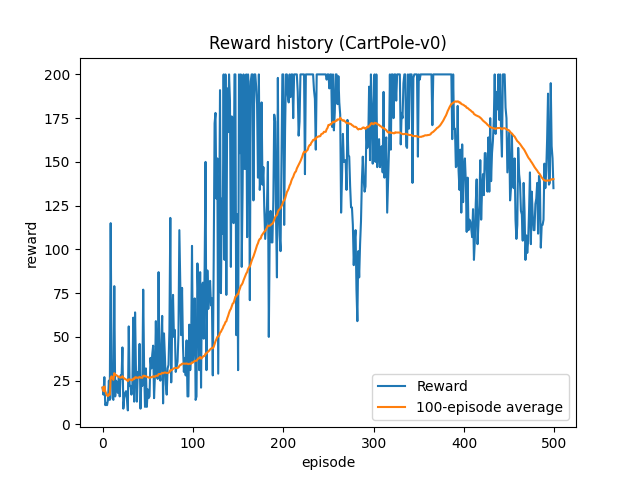
\includegraphics[scale=0.5]{exercise-1/report/img/task-1-training-200.png}
    \caption{Training result with 500 episodes and 200 max time steps per episode.}
    \label{fig:training-200}
\end{figure}

It is important to know that this is not a deterministic process, and that implies that the content of this plot is not the only possible training that the agent could have. But, as we can see in figure \ref{fig:training-200} the cumulative reward (equivalent to the maximum number of time steps that the pole was balanced), is increasing over the training episodes. Obtaining the maximum reward in some intervals between episodes 100 and 400. Also, the average reward has an increasing tendency over all the episodes except for the final 100 episodes. \\

After having trained the model, it was tested with a maximum of 500 timesteps per episode, and the obtained result was:

\begin{center}
    \texttt{Average test reward: 161.644 episode length: 161.644}
\end{center}

As we can see in this case, the agent did not generalized well, having an average test performance even worst than the parameter established for training which was 200 timesteps.

\subsection{Question 1.1}
\label{sec:question-1.1}
\textbf {
    Can the same model, trained to balance for 200 timesteps, also balance the pole for 500 timesteps? Briefily justify your answers.
}\\

The general answer to this question would be: yes it can. First of all, when the number of maximum time steps is increased, the main change is that the evaluation of the environment (in this case performed by \texttt{gym} using \texttt{env.step()}), is not going to consider the episode finalized (setting the \texttt{done} boolean variable to \texttt{true}) until the execution reaches 500 steps, or the pole falls.\\

So, as we previously trained the agent to balance the pole for 200 timesteps, theoretically it could continue doing it for more steps if it has generalized well during the training period. In practice, that is not happening in all the cases, mainly due to two reasons: On the one hand, the model is trained with 500 episodes, which could maybe not be enough for the generalization task, we can see that in Figure \ref{fig:training-200} where the variance between the average reward and some executions is really important. On the other hand, we have the maximum 200 train steps, which maybe is not enough too, we can see that also in the result of the test with 500 steps, which had as, a result, an average reward of 161.644. This result was even less than the 200 steps with which it was trained. 

\subsection{Task 2}
\label{sec:task-2}
\textbf {
    Repeat the experiment a few times, each time training the model from scratch with 200 time steps and testing it for 500 time steps.
}\\

The experiment was executed five different times from scratch, obtaining the corresponding training plots:

\begin{figure}[H]
   \begin{minipage}{0.32\textwidth}
     \centering
     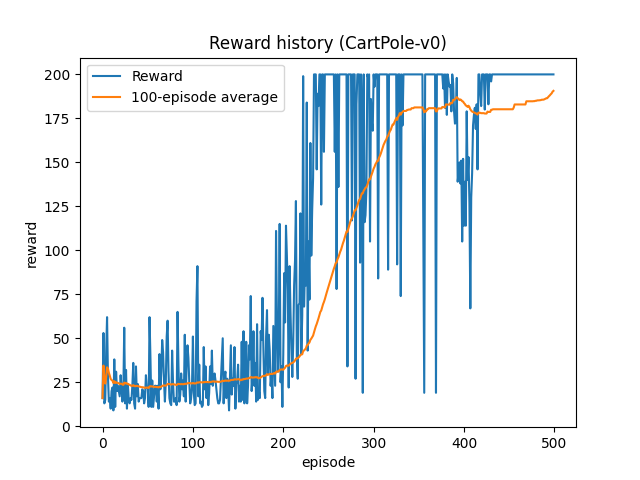
\includegraphics[width=\linewidth]{exercise-1/report/img/task-2-v1.png}
     \caption{First execution}
     \label{fig:task-2-v1}
   \end{minipage}\hfill
   \begin{minipage}{0.32\textwidth}
     \centering
     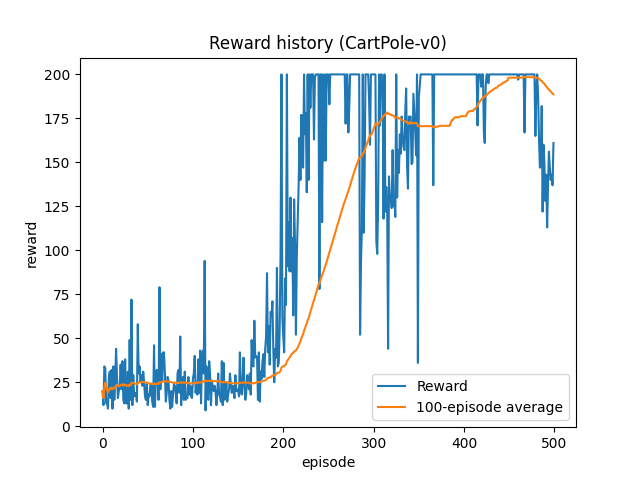
\includegraphics[width=\linewidth]{exercise-1/report/img/task-2-v2.png}
     \caption{Second execution}
     \label{fig:task-2-v2}
   \end{minipage}
   \begin{minipage}{0.32\textwidth}
     \centering
     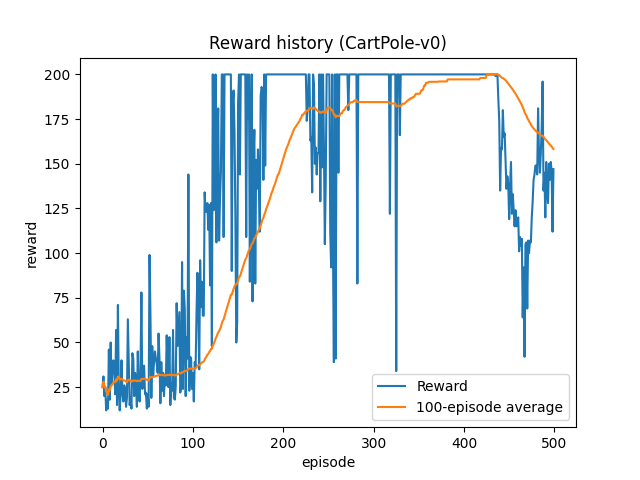
\includegraphics[width=\linewidth]{exercise-1/report/img/task-2-v3.png}
     \caption{Third execution}
     \label{fig:task-2-v3}
   \end{minipage}
\end{figure}

\begin{figure}[ht]
    \centering
   \begin{minipage}{0.48\textwidth}
     \centering
     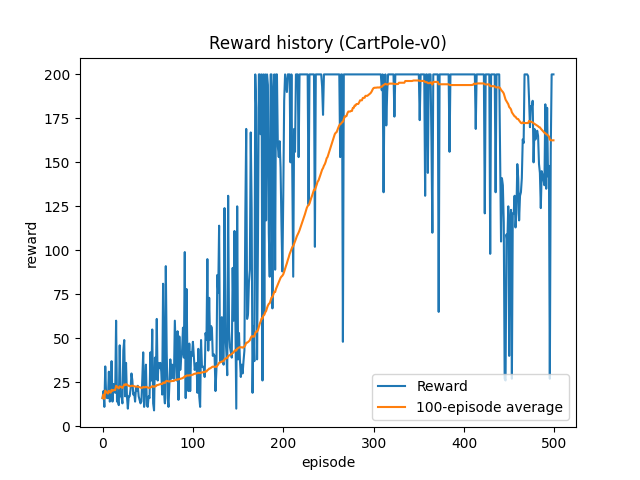
\includegraphics[width=0.68\linewidth]{exercise-1/report/img/task-2-v4.png}
     \caption{Fourth execution}
     \label{fig:task-2-v4}
   \end{minipage}\hfill
   \begin{minipage}{0.48\textwidth}
     \centering
     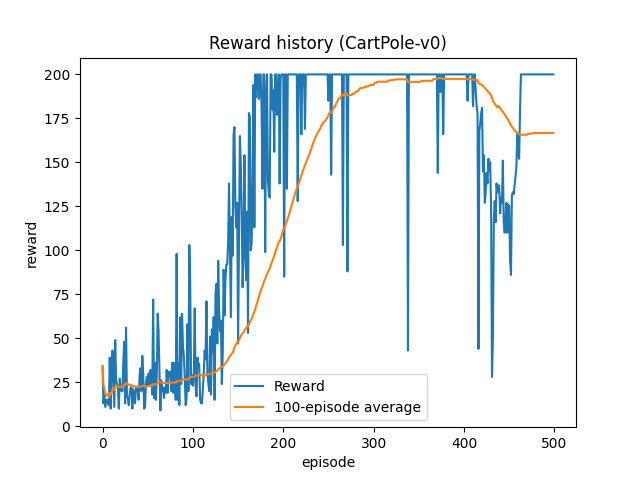
\includegraphics[width=0.68\linewidth]{exercise-1/report/img/task-2-v5.png}
     \caption{Fifth execution}
     \label{fig:task-2-v5}
   \end{minipage}
\end{figure}


Apart from the training plots, in the test phase, using 500 timesteps, we have obtained the following results stated in Table \ref{ref:rewards-table}.

\begin{table}[h]
\centering
\begin{tabular}{l|ccc}

\multicolumn{1}{l|}{Execution} & Figure                                      & \multicolumn{1}{l}{Average test reward} & \multicolumn{1}{l}{Episode length} \\ \hline
1                               & Figure \ref{fig:task-2-v1} & 497.632                                  & 497.632                             \\
2                               & Figure \ref{fig:task-2-v2} & 181.372                                  & 181.372                             \\
3                               & Figure \ref{fig:task-2-v3} & 138.476                                  & 138.476                             \\
4                               & Figure \ref{fig:task-2-v4} & 236.846                                  & 236.846                             \\
5                               & Figure \ref{fig:task-2-v5} & 299.016                                  & 299.016                            
\end{tabular}
\caption{Obtained rewards for the different executions}
\label{ref:rewards-table}
\end{table}

\subsection{Question 1.2}
\label{sec:question-1.2}
\textbf {
    Are the behavior and performance of the trained model the same every time? Analyze the causes briefly
}\\

As it was described in the previous section \ref{sec:question-1.1}, the system could achieve a better result than the 200 reward points that it was trained with, proof of that is the first execution, which achieved an average test reward of 497.632, which is almost the best possible reward that can be obtained. Apart from this execution, there have been others which has surpassed the barrier of the 200 reward points, such as the fifth and the sixth execution. 

It is remarkable to say that the behavior of the agent is not deterministic in any sense because the initial state is random each time the environment is initialized (when the episode ends), so the training has a different evolution each time that it is executed. The same happens with the test phase, that it is almost the same as the training phase but without the update of the outcome of the agent. \\

If we evaluate the performance in the graphic mode, we can do different observations. First of all, the trained agent learns to balance the pole even going to one side or the other, and that depends on the execution. Then, we can also observe that the agent learns to take advantage of the time and move from the border of the screen to finalize the episode in the established maximum time, in order to maximize the reward. Another relevant aspect is that the agent always follows a predefined direction (either goes left or right) and never changes the direction, even though this change could lead to more promising results (Figure \ref{fig:task-2-left} and Figure \ref{fig:task-2-right}).

\begin{figure}[ht]
    \centering
   \begin{minipage}{0.48\textwidth}
     \centering
     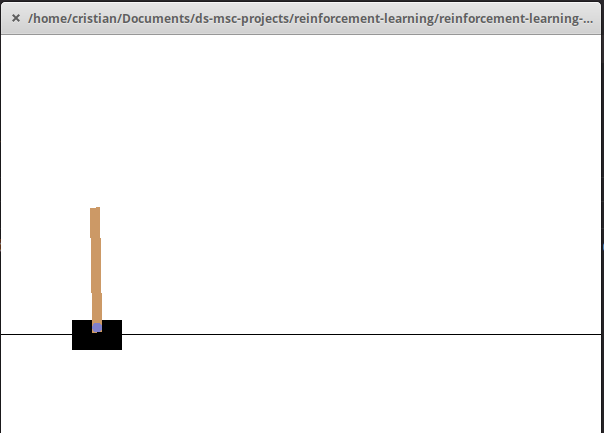
\includegraphics[width=0.7\linewidth]{exercise-1/report/img/task-2-left.png}
     \caption{Execution where the agent balanced the pole going to the left.}
     \label{fig:task-2-left}
   \end{minipage}\hfill
   \begin{minipage}{0.48\textwidth}
     \centering
     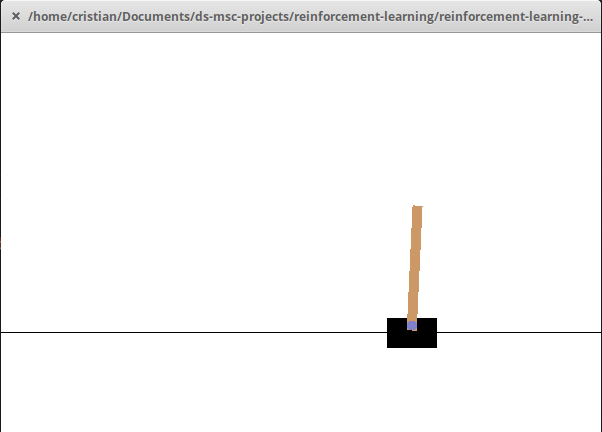
\includegraphics[width=0.7\linewidth]{exercise-1/report/img/task-2-right.png}
     \caption{Execution where the agent balanced the pole going to the right.}
     \label{fig:task-2-right}
   \end{minipage}
\end{figure}

\section{Repeatibility}
\label{sec:repeatibility}

\subsection{Question 2}
\label{sec:question-2}
\textbf {
    Why is this the case? What are the implications of this stochasticity, when it comes to comparing reinforcement learning algorithms to each other? Please explain.
}\\

In contrast to what happens in supervised methods of machine learning, in reinforcement learning the inputs that the intelligent system received are previously unknown, having only the capacity of observing some inputs that are initialized randomly and that are changed based on the effect that the actions taken by the agent produce. \\

\begin{figure}[H]
	\centering  
    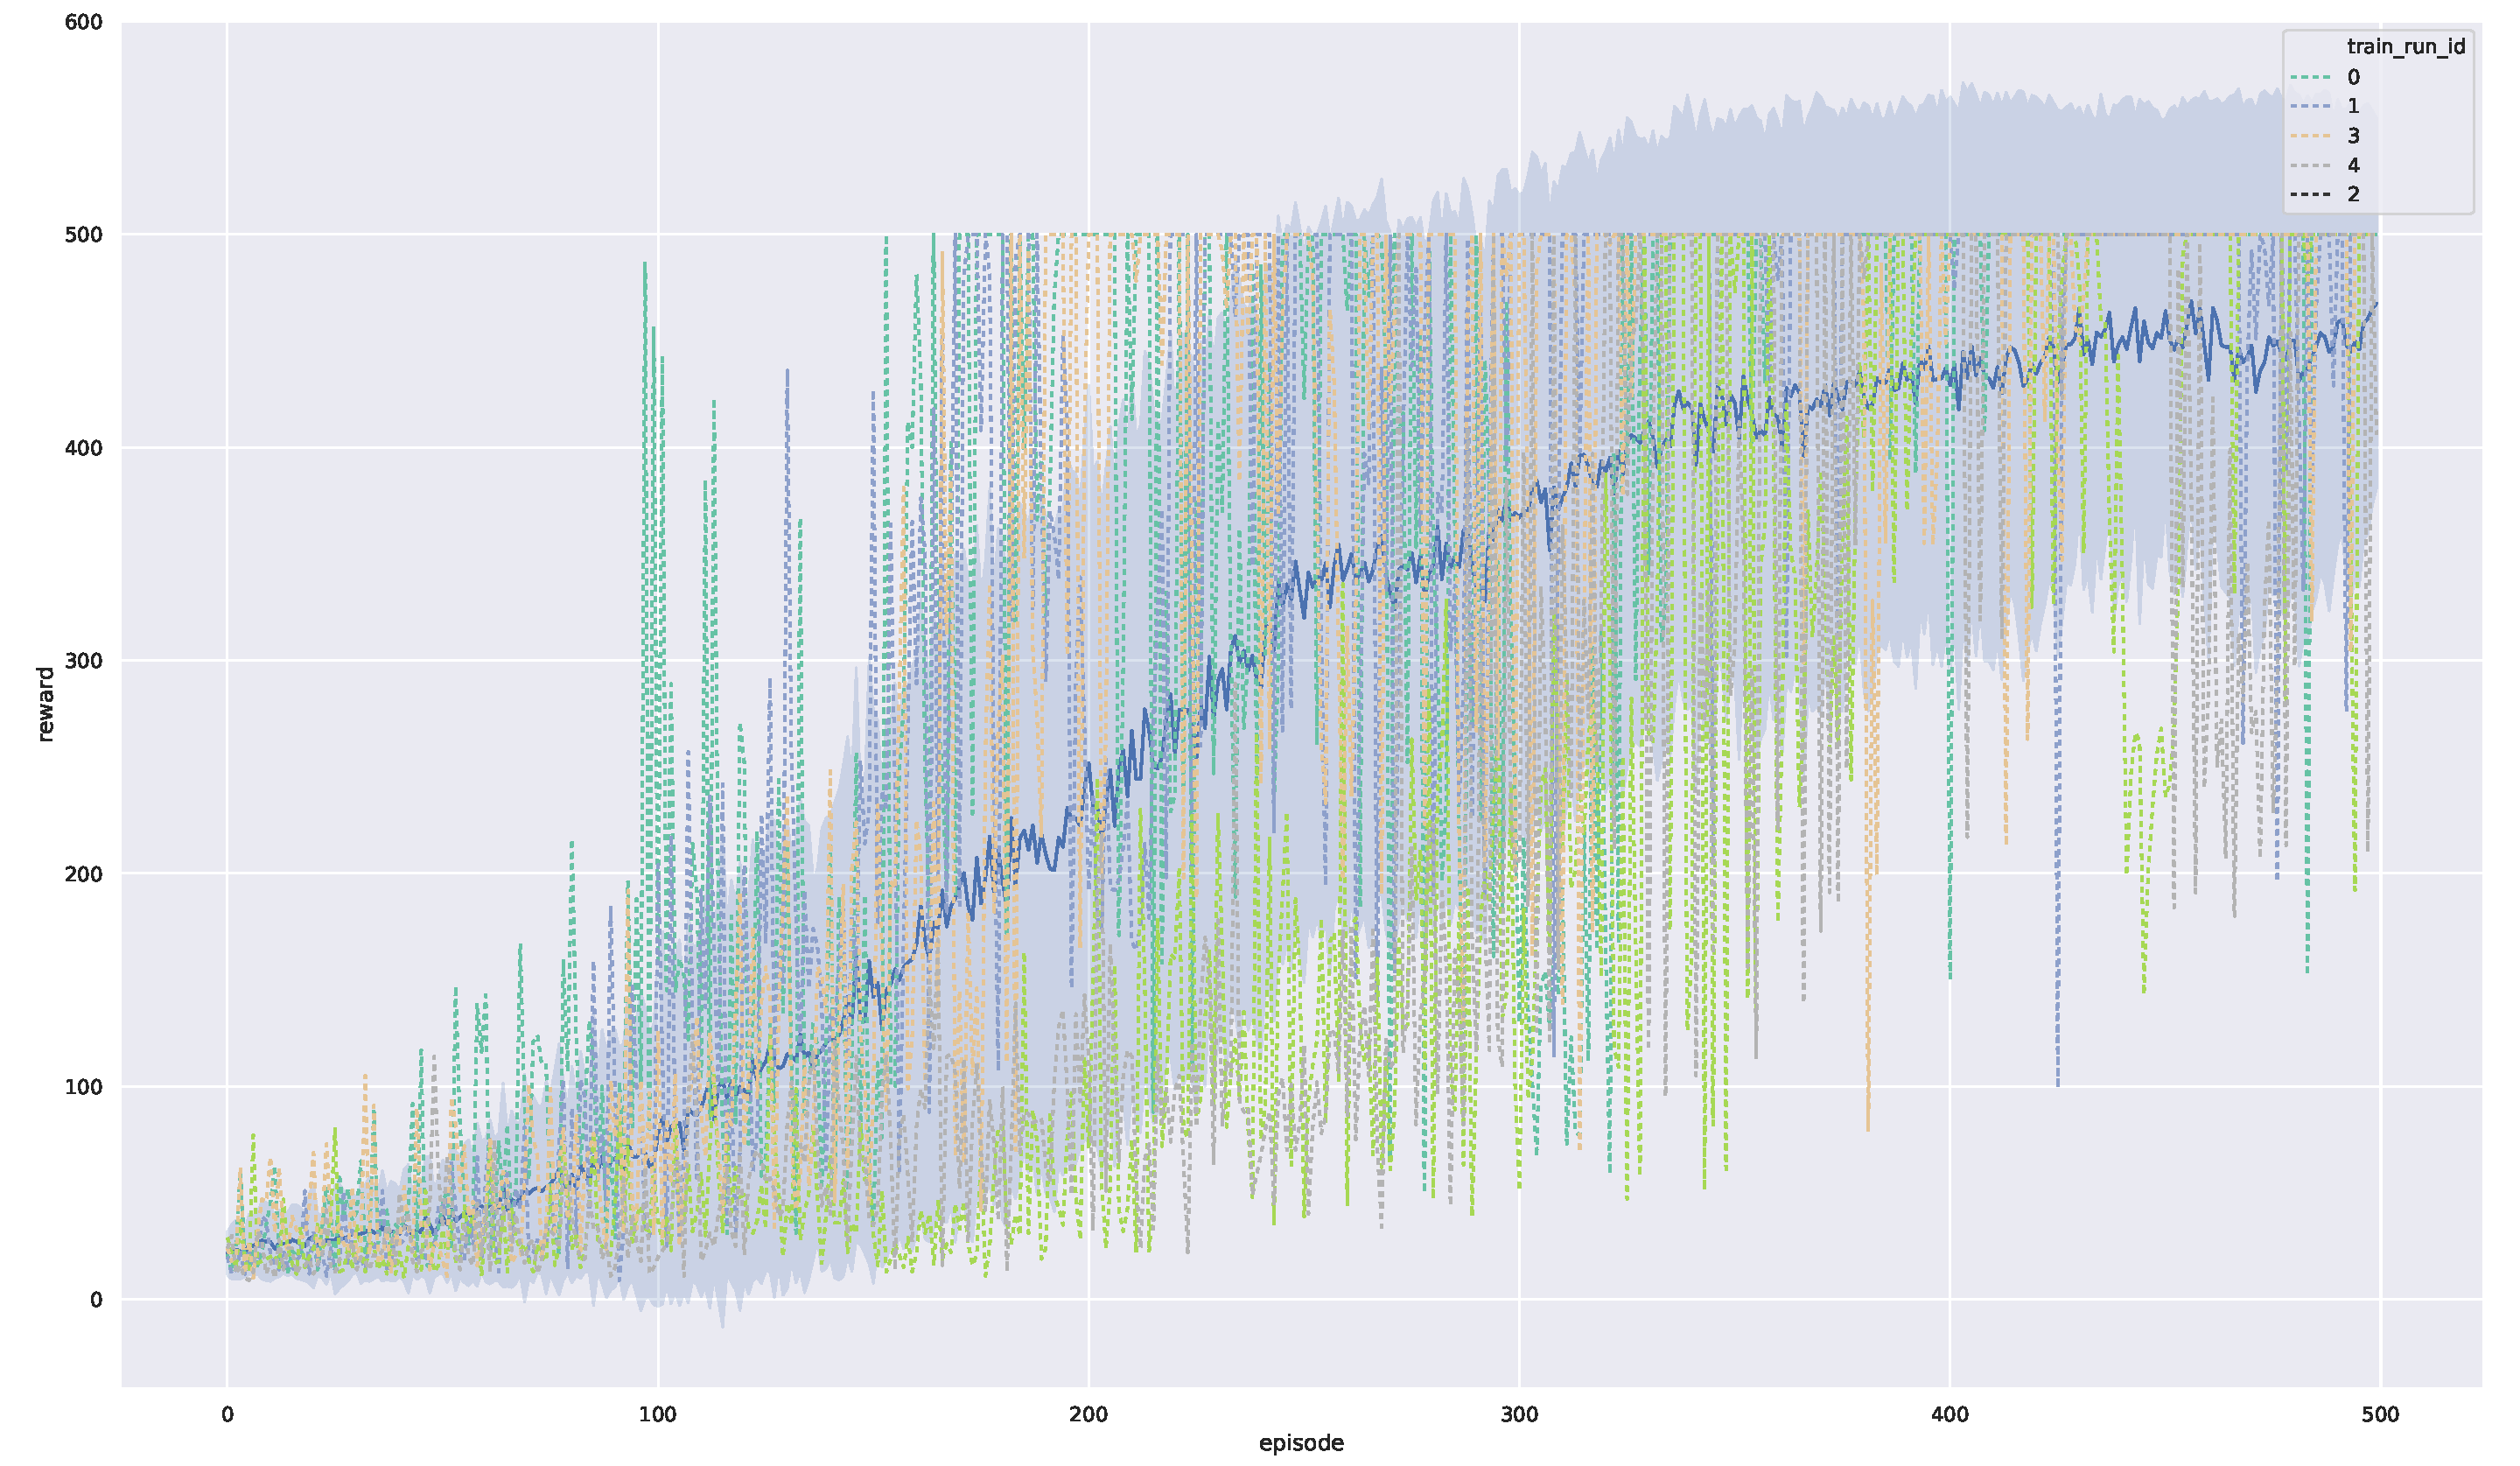
\includegraphics[width=0.6\columnwidth]{img/training.pdf}
	\caption{Execution of 100 independent trainings.}
	\label{question-2:fig}
\end{figure}


We can observe in figure \ref{question-2:fig} that even though there are many executions, the variety of the rewards obtained by different agents in those executions differ in a significant way between them. This is caused by the quantity of randomness that is present in the environment, not only with the initialization but also in how the model behaves (intelligent systems based on neural networks introduce an inevitable amount of randomness).\\

Having an agent trained in such as random environment inevitably creates difficulties for them in generalizing the underlying pattern, so the only way to evaluate the performance of those systems is the reward function, which varies drastically in different episodes. \\

As it was stated in \cite{nagendra2017comparison}, when we want to compare different reinforcement learning algorithms, it is difficult to know exactly which is going to be the convergence point, where we could distinguish which noise is produced by the environment and which is produced by the results of the algorithm.


\section{Reward functions}
\label{sec:reward-functions}

\subsection{Task 2}
\label{sec:reward-task-2}
\textbf {
    Write different reward functions to incentive the agent to learn the following behaviors:
}\\

\subsubsection{Balance the pole close to the center of the screen (close to $x = 0$)}
\label{sec:center}

Solving this question is equivalent to solve what is asked in section \ref{sec:center-point}, but for the specific case of $x=0$. For doing that, we have to design the reward function that could guide the position of the agent to the desired point. For doing that the approach followed could be better described with this diagram:

\begin{figure}[h]
    \centering
    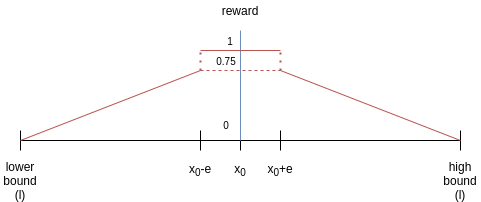
\includegraphics[scale=0.6]{exercise-1/report/img/diagrams/reward-diagram.png}
    \caption{Diagram of the reward given the position}
    \label{fig:reward}
\end{figure}

This diagram express the model that the reward will follow. When the actual position of the pole is in the interval specified between the desired point ($x_0$), and a threshold (denominated as $\epsilon$), we are going to return the maximum possible reward ($+1$). Then, when the position is in the interval between the lower bound and the beginning of the central interval, or between the end of the central interval and the upper bound, the reward is going to be obtained from the liner function proportionally specified between $0$ in the bounds and $0.75$ in the beginning of the central interval. \\

Calculating the equations of those intervals is easy, because they are simply the equation of the straight line that connects two different points, different from each interval (left and right). Those are the following equations:

\begin{minipage}{0.48\textwidth}
 \begin{center}
    \begin{equation}
         r = \frac{r_{max} \cdot (x - l)}{x_0-\epsilon-l}
    \end{equation}
 \end{center}
\end{minipage}\hfill
\begin{minipage}{0.48\textwidth}
\begin{center}
    \begin{equation}
        r = \frac{r_{max} \cdot (-x + h)}{h-(x_0 - \epsilon)}
    \end{equation}
 \end{center}
\end{minipage}
\\

It is important to mention that the parameter $r_{max}$ is the maximum reward obtained in the bounds of the central interval, in our case, this value was set to $r_{max} = 0.75$. Also, the value of $\epsilon$ established was $\epsilon=0.1$\\

This equations, should be translated to code, for this purpose, the following function was created:

\begin{pycode}
lower_bound = -1.5
higher_bound = +1.5
eps = 0.1
max_reward = 0.75

def proportional_reward(state, x0):
    x = state[0]

    if (x0 - eps) <= x <= (x0 + eps):
        return 1
    elif lower_bound <= x < (x0 - eps):
        denominator = x0 - eps - lower_bound
        return (max_reward / denominator) * x - ((max_reward * lower_bound) / denominator)
    elif (x0 + eps) < x <= higher_bound:
        denominator = higher_bound - (x0 + eps)
        return (-max_reward / denominator) * x + ((max_reward * higher_bound) / denominator)
    else:
        return 0
\end{pycode}

After have explained how the reward function was designed, we have to analyze the case of $x_0 = 0$, which is equivalent to center the pole in the screen. The training of this model was done using 500 timesteps in 1000 episodes, obtaining the following plot of the rewards:

\begin{figure}[h]
    \centering
    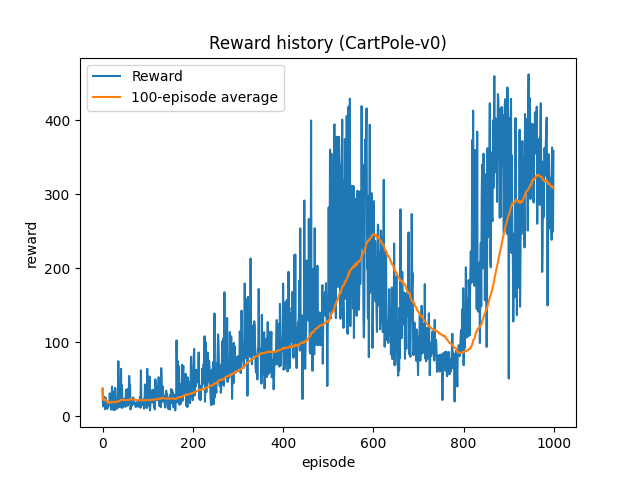
\includegraphics[scale=0.45]{exercise-1/report/img/rewards/center-0-500t-1000e-proportion.png}
    \caption{Reward function of the centering}
    \label{fig:rewards-1}
\end{figure}

The correspondent model obtained in this execution is \texttt{center-0-500t-1000e-proportional.ai}.

\subsubsection{Balance the pole in an arbitrary point of the screen ($x = x_0$), with $x_0$ passed as a command line argument
to the script.}
\label{sec:center-point}

The function designed for this question was already explained in section \ref{sec:center}. In this case, two different models were trained, the first one for center the model in $x = -1$ and the other for centering the model in $x=+1$. As in the previous section, both models were trained with 500 timesteps and 1000 episodes, obtaining the following plots of the rewards:

\begin{figure}[ht]
    \centering
   \begin{minipage}{0.48\textwidth}
     \centering
     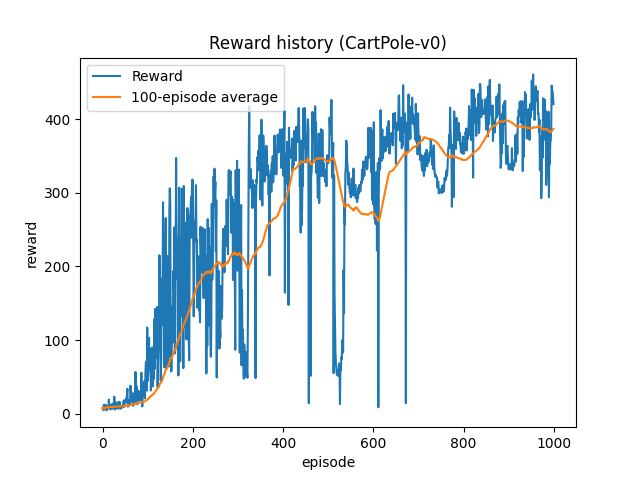
\includegraphics[width=0.7\linewidth]{exercise-1/report/img/rewards/center--1-500t-1000e-proportional.png}
     \caption{Reward plot for the model when $x=-1$}
     \label{fig:reard-1}
   \end{minipage}\hfill
   \begin{minipage}{0.48\textwidth}
     \centering
     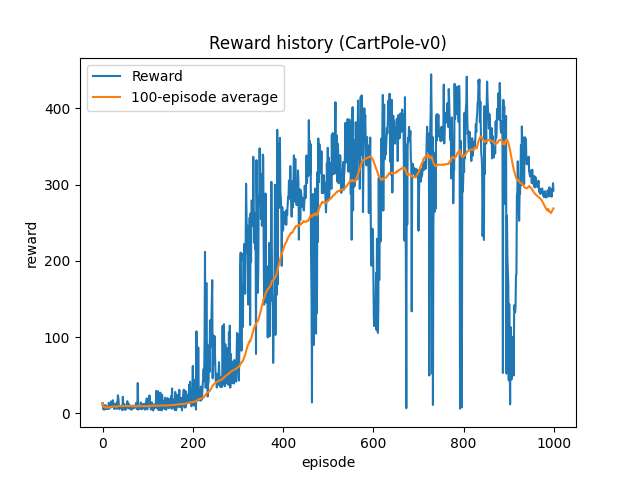
\includegraphics[width=0.7\linewidth]{exercise-1/report/img/rewards/center-1-500t-1000e.png}
     \caption{Reward plot for the model when $x=+1$}
     \label{fig:task-2-right}
   \end{minipage}
\end{figure}

As we can see, in both graphs, the average reward increases over time, following a period of stabilization in the final episodes of the training. The corresponding model files are: \texttt{center--1-500t-1000e-proportional.ai} and \texttt{center-+1-500t-1000e-proportional.ai}.

\subsubsection{Keep the cart moving from the leftmost to rightmost side of the track as fast as possible, while still
balancing the pole.}
\label{sec:balance}

The proposed solution to this reward function is inspired in the wave equation. The idea is that the velocity of the pole follows the trajectory described by the $sin$ function. In this wave function, the amplitude is by default $1$, so the objective is that given the timestamp, the function will perform which is the desired velocity. The equation is the following:

\begin{equation}
    v^* = sin(\frac{2\pi}{T}t)
\end{equation}


For achieving this, the following python function was elaborated:

\begin{pycode}
def balanced_reward(state, timesteps):
    period = 5
    eps = 0.05
    max_reward = 0.75

    v_ideal = np.sin((2 * np.pi / period) * timesteps)
    return proportional_reward(state[1], v_ideal, eps, max_reward)
\end{pycode}

This function calculates the ideal velocity that the pole should have in each time step and then compares the actual velocity following the equation described in section \ref{sec:center}. After training the model with 500 timesteps and 500 episodes, this is the obtained plot of the rewards: \\

\begin{figure}[h]
    \centering
    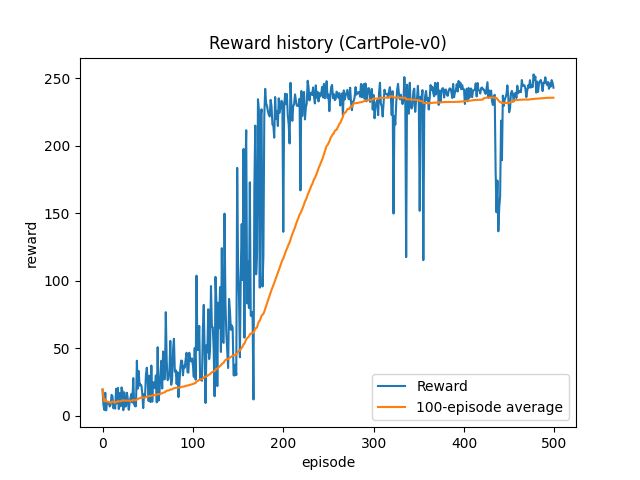
\includegraphics[scale=0.4]{exercise-1/report/img/rewards/balance-500t-500e.png}
    \caption{Plot of the rewards after 500 episoes of training}
    \label{fig:my_label}
\end{figure}

The graph shows a significant improvement in the reward obtained along the episodes, achieving an almost constant lines in the final episodes. The corresponding model of this function is \texttt{balanced-500t-500e.ai}.

\subsection{Task 3}
\label{sec:task-3-reward-viz}
\textbf {
    Let us visualize the third reward function
}\\

The execution of 10 parallel runs of the cart pole balance problem, shows this graph:

\begin{figure}[h]
    \centering
    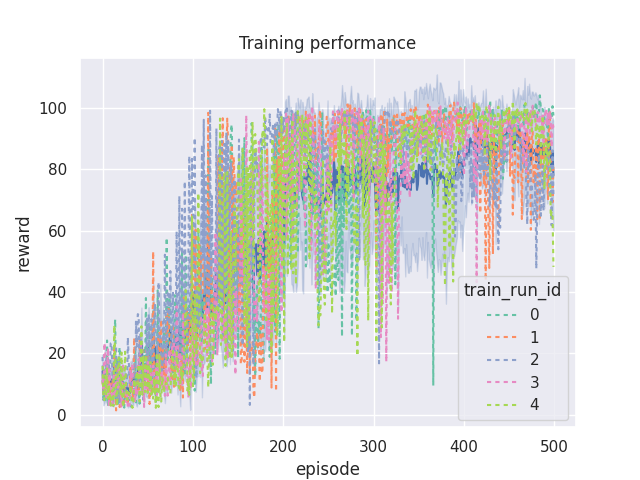
\includegraphics[scale=0.5]{exercise-1/report/img/rewards/Figure_1-multiple.png}
    \caption{10 executions with the reward function described in section \ref{sec:balance}}
    \label{fig:my_label}
\end{figure}

This plot shows also the problem of the high variance between different executions of the problem, but we can also observe than in the final phases of the training the variance is becoming less and the reward function is starting to stabilize, this is because the agent is learning the underlying pattern and maximizing the reward.

\subsection{Question 3}
\label{sec:question-3}
\textbf {
    What do you observe? What is the highest velocity the agent reaches?
}\\

When observing the execution of the cart pole with the third reward function, we can obtain different conclusions. First of all, the velocity of the pole is not adequate, because it goes slow and is not able to finish a complete oscillation in the 500 timestamps used for test. This happens because during the training phase, the agent learns how to maintain an average velocity in order to prevent the pole from falling. \\

\begin{figure}[h]
    \centering
    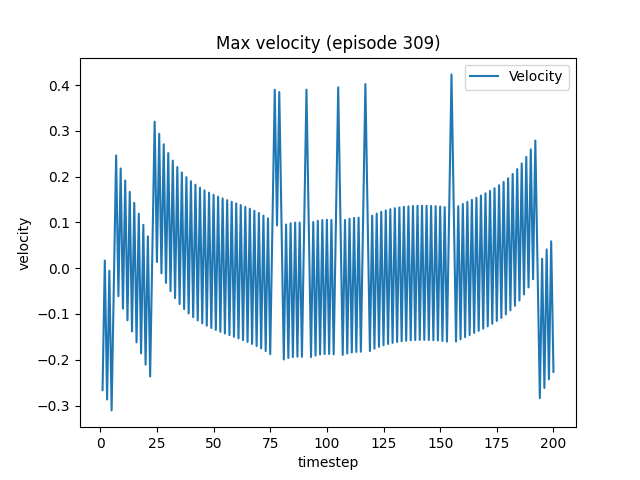
\includegraphics[scale=0.45]{exercise-1/report/img/rewards/velocity-1.png}
    \caption{Velocity diagram of the execution when the highest velocity was reached}
    \label{fig:velocity}
\end{figure}

This could be seen if we observe the velocity plot (Figure \ref{fig:velocity}) obtained in the episode when the maximum velocity is reached (\textbb{0.410}), in the episode 309 of the test. It shows that the velocity is approximately varying between $-0.2$ and $+0.2$, which indicates that the agent is always more or less following the same velocity, and do not \textit{risk} in increasing it. \\

We can conclude that the third reward function is not enough good, because even if it perform correctly the task, it does not do it in the desired velocity, and also it possibly uses unnecessary information for the calculation such as the timestamp of the current episode. 


\bibliographystyle{ieeetr}
\bibliography{template}  % Modify template with your bibliography name
\end{document}
